\documentclass[a4paper]{article}
%%%%%Paquetes%%%%%
\usepackage[T1]{fontenc}
\usepackage[utf8]{inputenc}
\usepackage[english]{babel}
\usepackage{amsmath,amssymb,eucal,mathrsfs}
\usepackage[svgnames,x11names]{xcolor}
\usepackage{colortbl}
\usepackage{Estilos/MiEstilo}
%\usepackage{Estilos/Informe}
\usepackage{amsmath}
\usepackage{times}
\usepackage{color}
\usepackage{listings}
\usepackage{graphicx}
\usepackage{caption}
\usepackage{float}
	\setcounter{tocdepth}{2} %Mostrar solo 3 niveles en el índice
		\makeindex	%índice de palabras
		\title{Computational Complexity\\ Assignment 1 }
		\author{Luis José Quintana Bolaño}
		\date{\today}

\begin{document}
	\maketitle
	\begin{abstract}
	    Brief analysis of the time complexity, both theoretically and empirically, of two previously designed Turing Machines for deciding binary palindromes and the equality of two binary numbers respectively. Aditionally, two equivalent machines for RAM model are proposed and compared.
  	\end{abstract}
	\section{Binary Palindrome Decider}
	    \subsection{Observed Time Complexity}
		    \begin{figure}[!h]
  			\centering
  			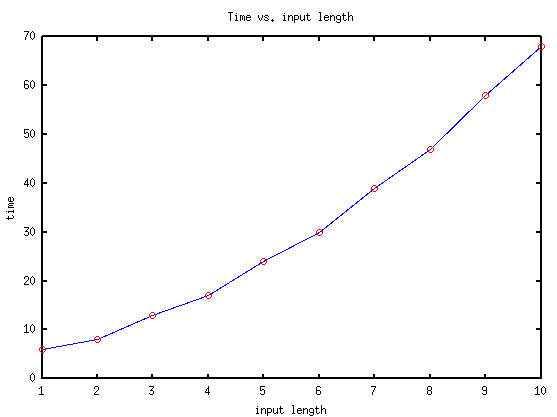
\includegraphics[width=0.55\textwidth,clip]{timepalindrometuring.png}
  			\caption{Plot of the time vs. input length for the turing machine implementation of the binary palindrome decider.}
  			\end{figure}
  		\subsection{Analysis}
  		    Assuming that each transition takes precisely one time unit, we conclude, upon close examination of the automaton, that the time function is $ T(n)=\frac1 2 n^2+\frac3 2 n+3+n\bmod2 $, and thus: $T(n)\in O(n^2)$
    \newpage
    \section{Binary Comparator}
        \subsection{Observed Time Complexity}
            \begin{figure}[!h]
  			\centering
  			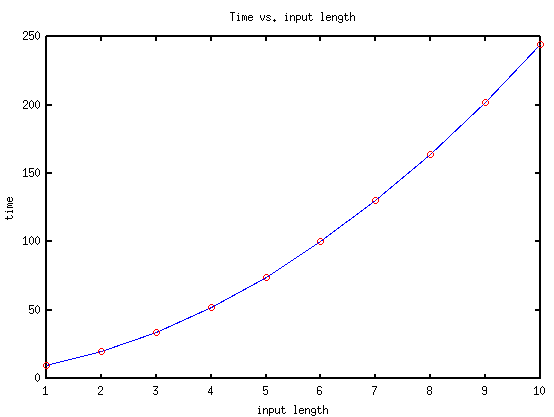
\includegraphics[width=0.55\textwidth,clip]{timecomparatorturing.png}
  			\caption{Plot of the time vs. input length for the turing machine implementation of the binary comparator.}
  			\end{figure}
  		\subsection{Analysis}
  		    Assuming that each transition takes precisely one time unit, we conclude, upon close examination of the automaton, that the time function is $ T(n)=2 n^2+4 n+4 $, and thus: $T(n)\in O(n^2)$
    \section{The RAM model}
        \subsection{Binary Palindrome Decider}
            \begin{figure}[!h]
  			\centering
  			\begin{tabular}{r|c|c|c|c|c|c|c|c|c|c|} \hline
  				input length  & 1 & 2 & 3 & 4 & 5 & 6 & 7 & 8 & 9 & 10 \\ \hline
  				time          & 35 & 39 & 56 & 60 & 77 & 81 & 98 & 102 & 119 & 123 \\ \hline
  		    \end{tabular} \\
  		    \end{figure}
  		    In this case, we can observe a time function $ T(n)\in O(n)$
        \subsection{Binary Comparator}
            \begin{figure}[!h]
  			\centering
  			\begin{tabular}{r|c|c|c|c|c|c|c|c|c|c|} \hline
  				input length  & 1 & 2 & 3 & 4 & 5 & 6 & 7 & 8 & 9 & 10 \\ \hline
  				time          & 34 & 49 & 64 & 79 & 94 & 109 & 124 & 139 & 154 & 169 \\ \hline
  		    \end{tabular} \\
  		    \end{figure}
  		    In this case, we can observe a time function $ T(n)=15n+19 $, and thus: $T(n)\in O(n)$
  		\subsection{Conclusion}
  		    In both machines the computations remain in polynomial time.
		
\end{document}
